\begin{ledgroupsized}[r]{120mm}%
\footnotesize%
\pstart%
\noindent\textbf{\"{U}berlieferung:}%
\pend%
\end{ledgroupsized}%
%  
\begin{ledgroupsized}[r]{114mm}%
\footnotesize%
\pstart \parindent -6mm%
\makebox[6mm][l]{\textit{L}}%
Auszüge mit Bemerkungen aus \cite{00326}\textsc{F.W. Nylandt}, \textit{Elementa physica sive Nova philosophiae principia}, den Haag 1669:
LH XXXV 14, 2 Bl. 103. 1 Bl. 2\textsuperscript{o}. 2 S.
Papier am rechten Rand beschädigt; dadurch Textverlust sowie Fehlstellen an den Diagrammen [\textit{Fig. 1}] und [\textit{Fig. 2}]. Ein
Wasserzeichen.\\%
Cc 2, Nr. 1367%
\pend%
\end{ledgroupsized}%
% \normalsize%
\vspace*{5mm}%
\begin{ledgroup}%
\footnotesize%
\pstart%
\noindent\footnotesize{\textbf{Datierungsgr\"{u}nde:} %
Leibniz spielt auf Nylandts naturphilosophisches Werk in \cite{01116}\textit{LSB} VI, 3 N. 16\textsubscript{1}, S.~220 an.
Dieses Stück soll zwischen Dezember 1675 und Mitte Februar 1676 entstanden sein (siehe die Datierungsbegründung ebd., S. 218).
Es ist daher zu vermuten, dass etwa zur gleichen Zeit Leibniz sich mit Nylandts \textit{Elementa physica} intensiv befasst und auch die vorliegenden Auszüge angefertigt hat.
Das Wasserzeichen bestätigt diese Vermutung.
Demgemäß lässt sich das vorliegende Stück auf die letzten Monate 1675 oder den Anfang 1676 datieren.}%
\pend%
\end{ledgroup}%
\vspace*{8mm}%
\count\Bfootins=1200
\count\Cfootins=1200
\count\Afootins=1200
\pstart%
\normalsize%
\noindent%
% [103~r\textsuperscript{o}]
[103~r\textsuperscript{o}] 
\cite{00326}\textit{Elementa \pgrk{F}ysica sive Nova philosophiae principia, ubi Cartesianorum principiorum falsitas ostenditur, ipsiusque errores ac paralogismi ad oculum demonstrantur ac refutantur a Francisco Wilhelmo libero Barone de Nuland etc.} Hagae\protect\index{Ortsregister}{Den Haag} Comitis ex officina Levyn van Dyck\protect\index{Namensregister}{\textso{Van Dyck}, Levyn} 1669. 12\textsuperscript{o}.
\pend%
\pstart%
(+ Nuland\protect\index{Namensregister}{\textso{Nylandt} (Nulandius), Franz Wilhelm Frhr. von 17. Jh.} Commandeur de Malthe\protect\index{Ortsregister}{Malta}, etc. il quitta les pays bas espagnols\protect\index{Ortsregister}{Spanische Niederlande} et sa religion et partie de ses biens, estant \'{e}pris d'amour d'une belle damoiselle, \`{a} la Haye\protect\index{Ortsregister}{Den Haag} depuis son frere luy a refus\'{e} son bien, il a eu proc\`{e}s avec luy sans finir. Il se jetta dans l'employ des armes. Estoit \`{a} Wesel\protect\index{Ortsregister}{Wesel} je croy qu'en qualit\'{e} de lieutenant colonel. Il mourut dans la fleur de son aage. Il avoit bien de la connoissance, m\^{e}me en chymie. Il entendoit bien l'Algebre. Il avoit cherch\'{e} les lignes des corps projetes qu'il pretendoit estre Analytiques et du 3 degrez. Il disoit avoir reduit la fortification \`{a} 3. theoremes principaux par le moyen de l'Analyse. +) Elegans ei satis dictio: sed ut appareat non nisi exercitium defuisse. 
\pend 
\pstart  Il met au commencement une lettre de Mons. Huygens\protect\index{Namensregister}{\textso{Huygens} (Hugenius, Ugenius, Hugens, Huguens), Christiaan 1629-1695}
26 April \edtext{1669.}{\lemma{1669}\Cfootnote{\glqq Extrait de la lettre de Monsieur Chrstiaen Huygens\grqq, in \cite{00326}\textsc{F.W. Nylandt}, \textit{Elementa physica}, den Haag 1669, Praefatio. Siehe \cite{01166}\textsc{C. Huygens}, Brief an Nylandt vom 26. April 1669 (\cite{00113}\textit{HO} VI, Nr.~1728, S.~420f.)}} \textit{La dispute touchant les idees et l'existence de Dieu par la voye qu'a pris M. des Cartes}\protect\index{Namensregister}{\textso{Descartes} (Cartesius, des Cartes), Ren\'{e} 1596-1650}
\textit{est tres obscure \`{a} mon avis.} \hspace{-1.2mm}\edtext{}{\lemma{\textit{\`{a} mon avis}.}\Cfootnote{\textsc{F.W. Nylandt}, \textit{Elementa physica}, Praefatio\cite{00326}.}} \textit{Je suis bien de vostre} avis, \textit{en ce que vous ne voulez pas, que la duret\'{e} se puisse separer de la nature d$\langle u~corps\rangle$ et Mons. }\textit{des Cartes}\protect\index{Namensregister}{\textso{Descartes} (Cartesius, des Cartes), Ren\'{e} 1596-1650}
\textit{en soutenant le contraire, et ne faisant consister le corps que dans l'estendue, $\langle$j'a$\rangle$y
tousjours concu que ce que j'entends par le vuide\protect\index{Sachverzeichnis}{vuide}, est la m\^{e}me chose que ce \edtext{qu'il $\langle$d$\rangle$it estre \edtext{corps.}{\lemma{\textit{corps.}}\Cfootnote{a.a.O., Praefatio.}}}{\lemma{qu'il}\Bfootnote{\textit{(1)} \textit{\textit{appelle co$\langle$rps$\rangle$}} \textit{(2)} \textit{$\langle$d$\rangle$it estre corps}. \textit{L}}}
Ce que vous dites contre le mouuement circulaire,\protect\index{Sachverzeichnis}{mouuement circulaire}
c'est \`{a} dire de la tendence du centre
me parois$\langle$t$\rangle$ fort paradoxe,
car \`{a} ce que j'ay pu comprendre,
c'est la nature du mouuement m\^{e}me
qui fait que les corps s'\'{e}loignent du centre par la circulation,\protect\index{Sachverzeichnis}{circulation}
et non pas la figure du canal, ou autre accident
\edtext{comme vous dites.}{\lemma{comme vous dites}\Cfootnote{Siehe \cite{01165}\textsc{F.W. Nylandt}, Brief an Huygens vom 16. Februar 1669 (\cite{00113}\textit{HO} VI, Nr.~1705, S.~366).}}
Et je vous prie de me dire, si ce \edtext{que vous adjoutez}{\lemma{\textit{que vous}}\Bfootnote{\textit{(1)}\ \textit{avez} \textit{(2)}\ \textit{adjoutez} \textit{L}}}
touchant un canal figur\'{e} en sorte qu'un corps qui est port\'{e} dedans circulairement s'approche avec rapidit\'{e} du centre, est une chose que vous ayez
\edtext{experiment\'{e}e.}{\lemma{\textit{experiment\'{e}e}.}\Cfootnote{\cite{00326}\textsc{F.W. Nylandt}, \textit{Elementa physica}, Praefatio.}}}
\pend% 
\pstart%
Cartesius\protect\index{Namensregister}{\textso{Descartes} (Cartesius, des Cartes), Ren\'{e} 1596-1650}
\textit{felix si ab immodica ambitione sibi temperare et nonnullas veritatis quas excusserat scintillas fovere clarioremque inde facem accendere
\edtext{potuisset.}{\lemma{\textit{potuisset.}}\Cfootnote{\cite{00326}a.a.O., S.~4f.}}}
\pend 
\count\Bfootins=1200
\count\Cfootins=1200
\pstart 
Creditum est ex nihilo nihil fieri,
et creationem superare captum mentis humanae,
verum re accurate inspecta videbimus revera materiam ex nihilo factam esse.
Nihil est non ens sine combinatione infiniti.
\textit{Ens finitum solum est objectum intellectus\protect\index{Sachverzeichnis}{intellectus} nostri
frustra contrarium asserente
\edtext{Cartesio.\protect\index{Namensregister}{\textso{Descartes} (Cartesius, des Cartes), Ren\'{e} 1596-1650}%
}{\lemma{Cartesio.}\Cfootnote{\cite{00326}a.a.O., S.~10.}}}
\textit{Finitum est medium}
\edtext{[\textit{proportionale}]}{\lemma{\textit{proportione}}\Bfootnote{\textit{L \"{a}ndert Hrsg. nach Vorlage}}}
\textit{inter nihilum et \edtext{infinitum.}{\lemma{\textit{infinitum}.}\Cfootnote{a.a.O., S. 11, gedruckte Marginalie.}}}
Eadem enim ratio nihili ad finitum, quae finiti ad infinitum.\protect\index{Sachverzeichnis}{infinitum}
Infinita ratio est
\textit{quae omni assignabili ratione major est, \textso{sub-infinita} quae minor.
Nihilum\protect\index{Sachverzeichnis}{nihilum} est quod ad aliquid rationem habet
\edtext{sub-infinitam}{\lemma{\textit{sub-infinitam}}\Cfootnote{\cite{00326}a.a.O., S.~11.}}}
(+~debebat dicere ad aliquod finitum. Nam et finitum talem habet ad infinitum.~+)
quia nullus punctorum numerus facit lineam,
nec ullus
\edtext{linearum lineam infinitam, hinc probare}{\lemma{linearum}\Bfootnote{\textit{(1)}\ punctum, hinc probat \textit{(2)}\ lineam [...] probare \textit{L}}}
conatur esse ut punctum ad lineam
adeoque lineam ad infinitam lineam,
adeoque lineam infinitam aequari quadrato sub linea finita,
quia rectangulum extremorum aequatur rectangulo sub
\edtext{mediis.}{\lemma{mediis.}\Cfootnote{\cite{00326}a.a.O., S.~12-14.}}
\textit{Continuum\protect\index{Sachverzeichnis}{continuum}
componi ex punctis
\edtext{infinitis.}{\lemma{infinitis.}\Cfootnote{\cite{00326}a.a.O., S.~15, gedruckte Marginalie.}}
Nihil et \textso{infinitum esse nomina }%
\edtext{\textso{relativa.}}{\lemma{\textit{\textso{relativa}}.}\Cfootnote{\cite{00326}a.a.O., S.~15, gedruckte Marginalie.}}
Punctum et lineam in ratione superficiei aequalia esse},
quia utrumque ejus ratione \edtext{nihilum.}{\lemma{nihilum.}\Cfootnote{\cite{00326}a.a.O., S.~16.}}
Hinc facile
\edtext{[solvitur]}{\lemma{solvitur}\Bfootnote{\textit{erg. Hrsg. nach Vorlage}}}
\textit{Galilaei\protect\index{Namensregister}{\textso{Galilei} (Galilaeus, Galileus), Galileo 1564-1642}
paradoxum, quod centrum aequale
\edtext{peripheriae}{\lemma{peripheriae}\Cfootnote{\cite{00326}a.a.O., S.~17.
Siehe \cite{00050}\textsc{G.~Galilei}, \title{Discorsi}, Leiden 1638, S.~29 (\cite{00048}\title{GO} VIII, S.~75).}}};
nam areas areis comparando ostendit aream puncti
\textit{aequari areae peripheriae circuli, qui apex est cylindri
\edtext{multati,}{\lemma{multati,}\Cfootnote{\cite{00326}\textsc{Nylandt}, \textit{Elementa physica}, S.~17.}}}
\edtext{ut superficies jam est ad}{\lemma{ut}\Bfootnote{\textit{(1)}\ linea est ad \textit{(2)}\ superficies jam est ad \textit{L}}}
solidum, ita corpus vel solidum mathematicum est \edtext{ad physicum.}{\lemma{ad physicum.}\Cfootnote{\cite{00326}a.a.O., S.~18.}}
Et ex infinitis punctis in unum densatis fit punctum \pgrk{f}ysicum.
\pend 
%\newpage
\pstart  Poterat Cartesius\protect\index{Namensregister}{\textso{Descartes} (Cartesius, des Cartes), Ren\'{e} 1596-1650}
Vacuum corpus \pgrk{f}ysicum vocare, si modo \textit{non sub eo nomine obtrusisset solem\protect\index{Sachverzeichnis}{sol}, stellas\protect\index{Sachverzeichnis}{stella}, Mund$\langle$um$\rangle$.}\edtext{}{\lemma{\textit{Mund$\langle$um$\rangle$}.}\Cfootnote{a.a.O., S. 29.}} De Vacui \textit{necessitate in natura persuasi sumus}\edtext{}{\lemma{\textit{sumus}}\Cfootnote{a.a.O., S. 30.\cite{00326}}} (+~non adjicit rationem +). 
\pend 
\pstart%
Corpus physicum factum ex densatis in unum infinitis mathematicis.
\textit{Duo corpora \pgrk{f}ysica naturaliter impenetrabilia esse,}
quia enim vi infinita utrumque densatum sit,
\textit{nulla vi finita in eundem locum compingi, id est infinities rursus densari}
posse patet.
Hinc esse vim elas$\langle$ticam,$\rangle$
quod co$\langle$rpo$\rangle$ra novae densationis\protect\index{Sachverzeichnis}{densatio}
\edtext{impatientia}{\lemma{impatientia}\Cfootnote{a.a.O., S.~32.\cite{00326}}}
(+~hic labitur:
\edtext{nam si densationi contraria}{\lemma{nam si}\Bfootnote{\textit{(1)}\ densationis impatiens \textit{(2)}\ densationi contraria \textit{L}}}
$\langle$-- -- --$\rangle$ densari corpus
cum superatur ejus vis Elastica.
Nota etiam ejus ratiocinationi de impenetra$\langle$bilitate\protect\index{Sachverzeichnis}{impenetrabilitas}
corporis o$\rangle$bjici posse,
\edtext{quod vis quae corpus}{\lemma{quod}\Bfootnote{\textit{(1)}\ corpus \textit{(2)}\ vis quae \textit{(a)}\ aliud \textit{(b)}\ corpus \textit{L}}}
a corpore penetrari facit infinita sit,
quia $\langle$-- --$\rangle$ ex$\langle$pand$\rangle$et se alio corpore densato~+).
\pend%
\count\Bfootins=1000
\count\Cfootins=1000
\pstart%
(Pag. 38. nobis \textit{Venerem vel in meridie videre non semel
\edtext{contigit.}{\lemma{contigit.}\Cfootnote{a.a.O., S.~38.\cite{00326}}}}
Caeruleus coeli color est
\edtext{aeris.}{\lemma{aeris.}\Cfootnote{a.a.O., S.~39.\cite{00326}}})
Materia\protect\index{Sachverzeichnis}{materia} semel densata movenda fuit ab autore,
et in atomos\protect\index{Sachverzeichnis}{atomus} discerpenda.
Vacui plurimum inter \edtext{atomos.}{\lemma{atomos.}\Cfootnote{a.a.O., S.~43-45.\cite{00326}}}
Cartesius\protect\index{Namensregister}{\textso{Descartes} (Cartesius, des Cartes), Ren\'{e} 1596-1650}
alicubi vacui\protect\index{Sachverzeichnis}{vacuum} necessitatem aliis verbis
\edtext{agnovit.}{\lemma{agnovit.}\Cfootnote{a.a.O., S.~47.\cite{00326}}}
\textit{Fatendum $\langle$aliqui$\rangle$d in mo$\langle$tu$\rangle$ isto reperiri,
quod mens quidem nostra percipit verum esse,
sed tamen quo pacto fiat non comprehendi$\langle$t,$\rangle$
nempe divisionem quarundam particularum in infinitum sive indefinitum,
atque in tot partes ut nullam cogitatione\protect\index{Sachverzeichnis}{cogitatio}
determinare possimus tam exiguam,
quin intelligamus ipsam in alias adhuc rursu$\langle$s$\rangle$ reapse esse
\edtext{divisam.}{\lemma{divisam.}\Cfootnote{a.a.O., S. 47f.\cite{00326}}}}
\edtext{Haec ille[.]}{{\lemma{Haec ille}\Bfootnote{\textit{erg. L}}}%
{\lemma{Haec ille}\Cfootnote{Siehe \cite{00035}\textsc{R. Descartes}, \textit{Principia philosophiae},
pars II, §~5ff., Amsterdam 1644, S.~35ff. (\cite{00120}\textit{DO} VI, S.~42ff).}}}
Materiam\protect\index{Sachverzeichnis}{materia} autem esse \textit{infinities comminutam}
\edtext{[\textit{id}]}{\lemma{\textit{id}}\Bfootnote{\textit{gestr. L, wieder gültig macht Hrsg. nach Vorlage}}}
\textit{est in puncta sive nihil redactam}
\edtext{esse}{\lemma{esse}\Cfootnote{\cite{00326}\textsc{F.W. Nylandt}, \textit{Elementa physica}, S.~48.\cite{00326}}}
(+~\Denarius\ nam aliud est infinities comminutum aliud infinities rarum$\langle$.~+)$\rangle$
$\langle$--~--$\rangle$ densitas\protect\index{Sachverzeichnis}{densitas} differt a duritie,\protect\index{Sachverzeichnis}{durities}
ut mercurius\protect\index{Sachverzeichnis}{mercurium} et vitrum.\protect\index{Sachverzeichnis}{vitrum}
Nam in illo \edtext{parum}{\lemma{illo}\Bfootnote{\textit{(1)}\ bene \textit{(2)}\ parum \textit{L}}} intercedit vacui,
$\langle$at inco$\rangle$haerent singula.
In vitro cohaerent singula,
sed figuras habent vacuum\protect\index{Sachverzeichnis}{vacuum} non
\edtext{excludentes.}{\lemma{excludentes.}\Cfootnote{a.a.O., S.~51.\cite{00326}}}
Nos p$\langle$onimus at$\rangle$omos cum superficietenus se tangunt in unum corpus coalescere,
cum per puncta aut li$\langle$neas$\rangle$,
tunc m$\langle$agis flu$\rangle$idas, et hoc duriora esse corpora quo latiores
\edtext{[superficies]}{{\lemma{superficiores}\Bfootnote{\textit{L \"{a}ndert Hrsg.}}}{\lemma{[superficies]}\Cfootnote{a.a.O., S.~54f.\cite{00326}}}}
\edtext{(+~verum hoc sit}{\lemma{(+\hspace{-1.2mm}\phantom)}\Bfootnote{\textit{(1)}\ videri \textit{(2)}\ verum hoc sit \textit{L}}}
in systemate $\langle$--$\rangle$ata$\langle$--$\rangle$
rerum connexione\protect\index{Sachverzeichnis}{connexio}, cum quasi tabulae premuntur~+).
Fermentatio\protect\index{Sachverzeichnis}{fermentatio} plerumque
\textit{ex concursu $\langle$salium$\rangle$ lixivialium, et acidorum
\edtext{solutorum.}{\lemma{solutorum.}\Cfootnote{a.a.O., S.~57.\cite{00326}}}}
Salia lixivialia\protect\index{Sachverzeichnis}{salia lixivialia} putat constare
\textit{ex Elateribus\protect\index{Sachverzeichnis}{elater} vi contor$\langle$tis$\rangle$
ac te$\langle$nui$\rangle$ vi$\langle$nculo$\rangle$ $\langle$ne$\rangle$ explicari possint
ligatis, ab acidis,\protect\index{Sachverzeichnis}{acidum}}
quasi \textit{gladiolis\protect\index{Sachverzeichnis}{gladiolus} haec vincula
\edtext{incidi}{\lemma{\textit{incidi}}\Cfootnote{a.a.O., S.~58.\cite{00326}}}}
et e $\langle$--~--~--$\rangle$
\textit{Ens infinitum sive} summe \textit{perfectum nullo modo} intelligimus
nisi $\langle$idea nega$\rangle$tiv$\langle$a,$\rangle$ ad DEum perveniendum \edtext{a posteriori.}{\lemma{a posteriori.}\Cfootnote{a.a.O., S.~62.\cite{00326}}} \textit{Materia creata a solo DEo moveri potuit}\edtext{}{\lemma{\textit{potuit}}\Cfootnote{a.a.O., S. 63, gedruckte Marginalie.\cite{00326}}} hoc $\langle$mo$\rangle$do
%
[103~v\textsuperscript{o}]
%
ut eam tantum finita sua vi percuteret, sed finita. Nam si impetu infinito impulisset rursus in nihilum id est puncta redigisset, at finito impetu, in diversas figuras dissiliret, variis formis praeditas, quae variis formis praeditae sibi cohaerebunt. Uti massa \textit{ex vitro solida ingenti malleo\protect\index{Sachverzeichnis}{malleus} percussa in minimas particulas dissilire cogitur, et quo malleus saltem vis percutiens fuerit major,}
\edtext{[\textit{eo}]}{\lemma{etiam}\Bfootnote{\textit{L ändert Hrsg. nach Vorlage}}}
\textit{particulae\protect\index{Sachverzeichnis}{particulum} minores
\edtext{efficiuntur.}{\lemma{efficiuntur.}\Cfootnote{\cite{00326}a.a.O., S.~63f.}}}
Quies
\textit{rationem ad motum habet infinitam}[,]
\textit{quemadmodum nullum datur corpus cui nullum sit vacuum interspersum,
ita nullus datur motus cui nulla sit quies interspersa.}
Si tamen id fieret, foret motus
\edtext{instantaneus.}{\lemma{instantaneus.}\Cfootnote{a.a.O., S.~65f.\cite{00326}}}
\textit{Quies est motus infinite
\edtext{tardus}{\lemma{tardus}\Cfootnote{\cite{00326}a.a.O., S.~66, gedruckte Marginalie.}}} (+ \edtext{Des-arguesio\protect\index{Namensregister}{\textso{Desargues} (Des Argues), Girard (G\'{e}rard, Gaspard) 1591-1661} linea est punctum infinite motum}{\lemma{Des-arguesio [...] motum}\Cfootnote{Nicht nachgewiesen.}} +). 
Motus in linea recta. Corpus impellit aliud corpus in linea
\edtext{ad planum}{\lemma{ad}\Bfootnote{\textit{(1)}\ motum \textit{(2)}\ planum \textit{L}}}
recipientis \edtext{perpendiculari.}{\lemma{perpendiculari.}\Cfootnote{a.a.O., S.~70.\cite{00326}}}
Duobus modis ait fieri posse motum circularem,
(quem ait non nisi per accidens oriri in
\edtext{natura,}{\lemma{natura,}\Cfootnote{a.a.O., S.~70f.\cite{00326}}}$\lbrack)\rbrack$
uno, dum corpus in uno puncto fixum, in alio \edtext{impellitur;}{\lemma{impellitur;}\Cfootnote{a.a.O., S.~71f.\cite{00326}}}
alterum dum corpus in aliud incidit in linea quae
\edtext{cum linea
\textit{a puncto contactus ad centrum gravitatis\protect\index{Sachverzeichnis}{centrum gravitatis} ducta angulum
\edtext{facit.}{\lemma{\textit{facit}}\Cfootnote{\cite{00326}a.a.O., S.~72.}}}%
}{\lemma{cum}\Bfootnote{\textit{(1)}\ ejus centro gravitatis angulum facit. (\Denarius) \textit{(2)}\ linea [...] \textit{facit.} \textit{L}}}
\pend
\pstart 
%\begin{wrapfigure}[15]{l}{0.58\textwidth}  
%\vspace{-5mm}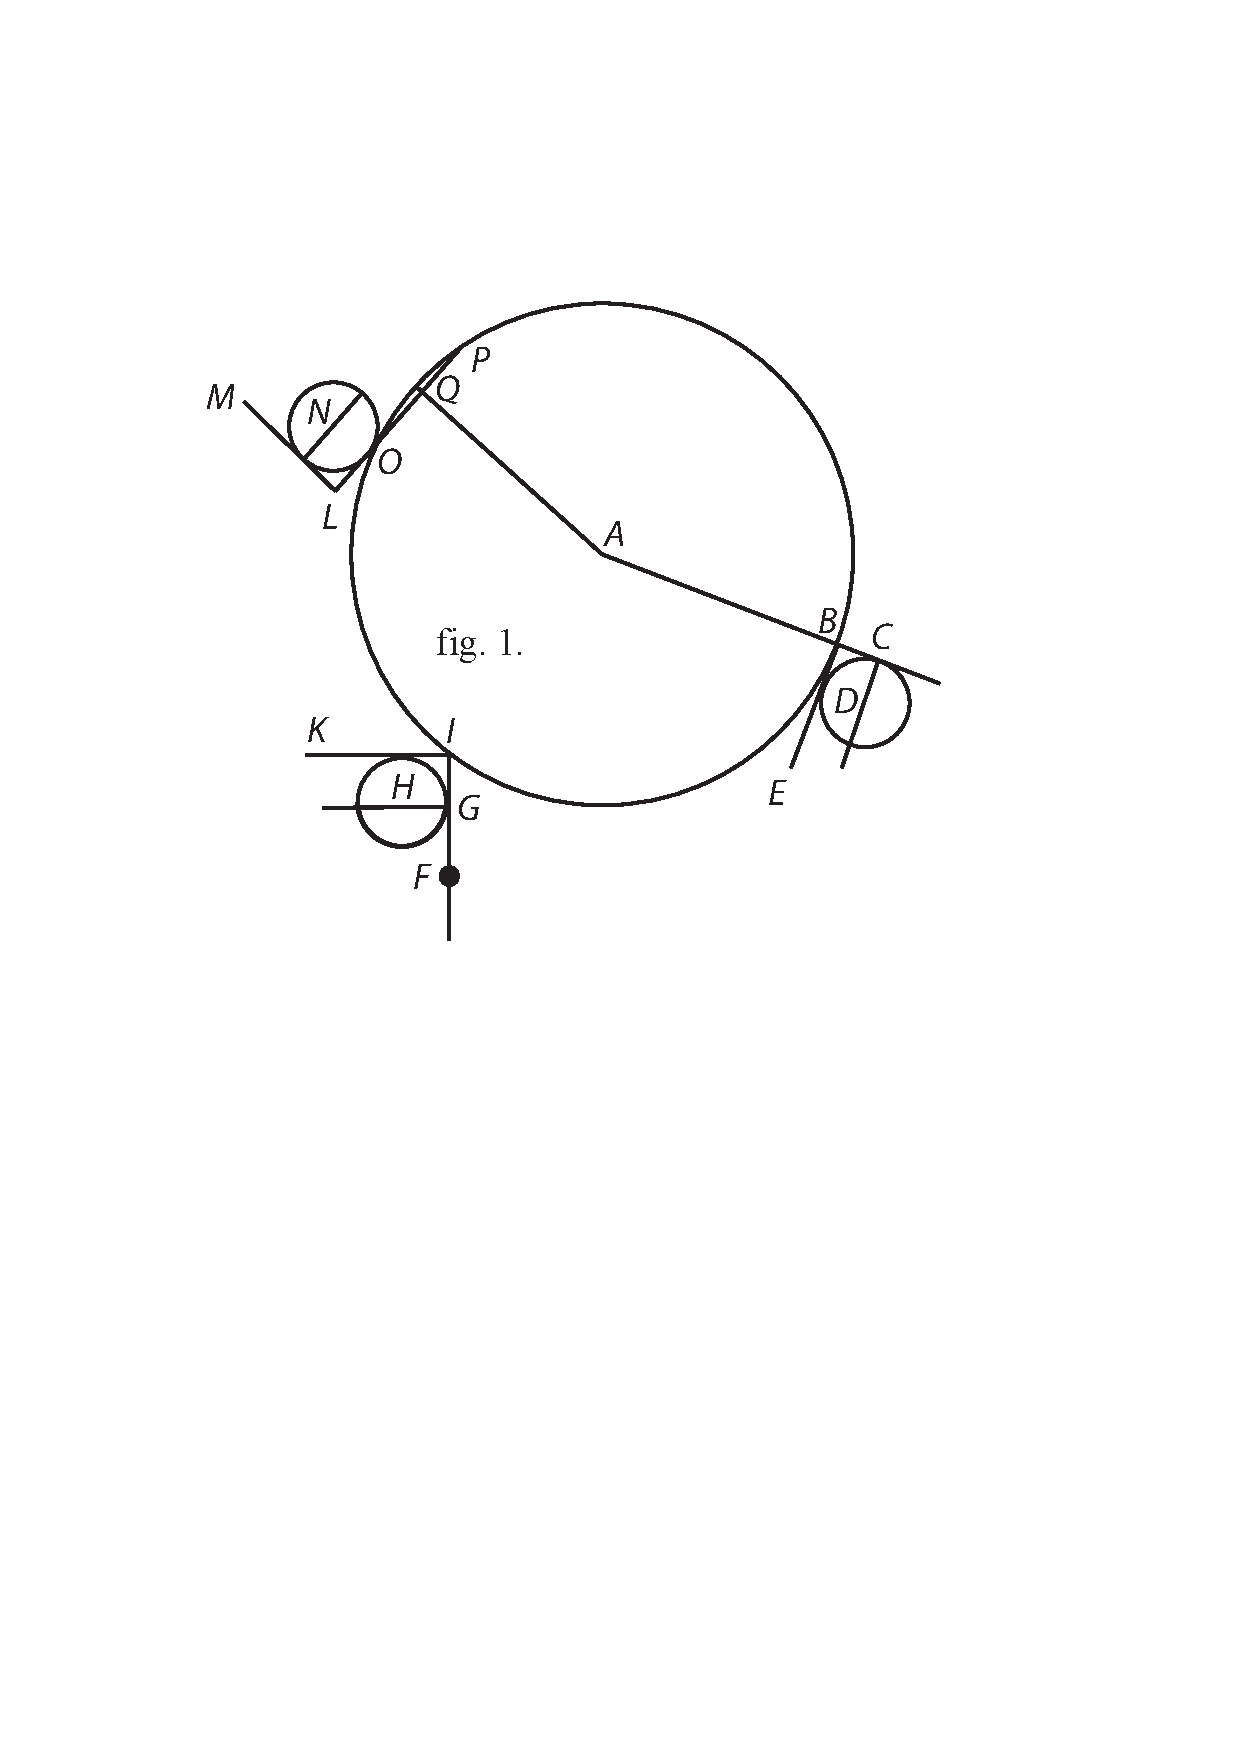
\includegraphics[width=0.58\textwidth]{images/LH0351402_103v-d1.pdf}\\
%%\centering [\textit{Fig. 1}]
%\end{wrapfigure} 
\textit{Agatur rota BGOP supra centrum A secundum puncta
\edtext{B G O.}{\lemma{B G O.}\Cfootnote{\cite{00326}a.a.O., S.~75.}}}
\edtext{Sit}{\lemma{Sit}\Bfootnote{\textit{erg. L}}}
\edtext{[\textit{EBA}]}{\lemma{\textit{ECA}}\Bfootnote{\textit{ L ändert Hrsg. nach Vorlage}}}
ang. rectus. \textit{CD} parallela \textit{EB}. \textit{D} centrum corporis resistentis ipsi \textit{EB} quae et tangens circuli; corpus \textit{D} liberatum procedet in recta \textit{BE} producta, adeoque a centro recedet. Si \textit{IF} angulum faciat recto majorem ad circulum, ad quem \edtext{\textit{IF}}{\lemma{\textit{IF}}\Bfootnote{\textit{erg. L}}} in puncto contactus perpendicularis \textit{IK} et \textit{GH} per \textit{H} centrum gravitatis\protect\index{Sachverzeichnis}{centrum gravitatis} 
corporis
\edtext{[\textit{H}]}{\lemma{\textit{G}}\Bfootnote{\textit{ L ändert Hrsg. nach Vorlage}}}
transit; ibit corpus \textit{H} liberatum in continuata \textit{GH} et rursus \edtext{recedet}{\lemma{rursus}\Bfootnote{\textit{(1)}\ accedet \textit{(2)}\ recedet \textit{L}}} a centro. Sed si \textit{ML} angulum faciat minorem recto, tunc corpus \textit{N} 
\pend
\count\Bfootins=1200
\count\Cfootins=1200
\newpage
\pstart
\centering
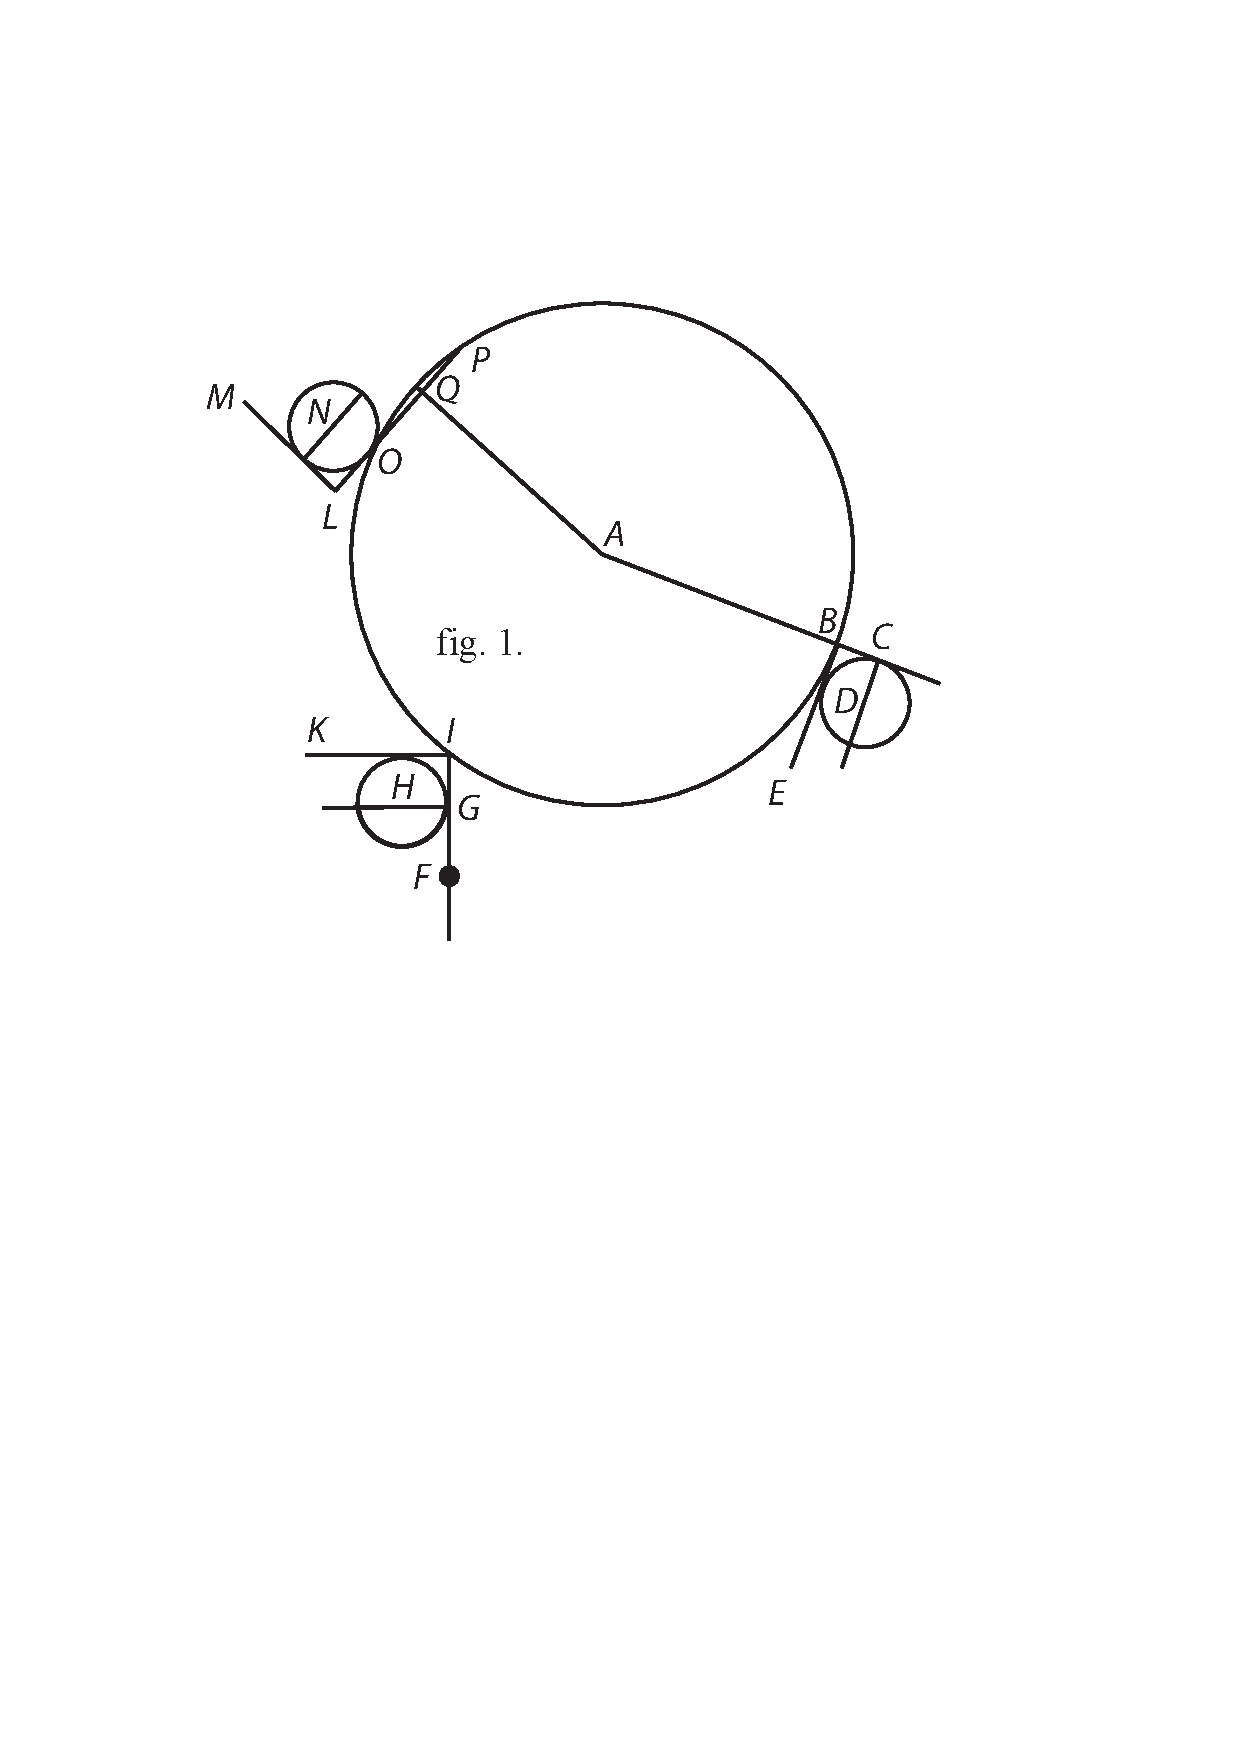
\includegraphics[width=0.56\textwidth]{images/LH0351402_103v-d1.pdf}\\
\centering [\textit{Fig. 1}]\edtext{}{\lemma{\hspace*{1,7mm}[\textit{Fig. 1}]}\killnumber\Cfootnote{Vgl. die Abbildung \cite{00326}a.a.O., S.~75.}}
%%\centering [\textit{Fig. 1}]
\pend
\vspace{1em}
\pstart\noindent cujus \setline{1}centrum \textit{N} impellet in recta ad \textit{ML} \edtext{perpendiculari [\textit{LOQP}] quo ad}{\lemma{}%
\Bfootnote{perpendiculari \textbar\ \textit{NOQP} \textit{\"{a}ndert Hrsg. nach Vorlage} \textbar\ \textit{(1)}\ ubi a \textit{(2)}\ quo ad \textit{L}}}
centrum accedet. Inde ab \textit{O} usque
\edtext{ad \textit{Q}.}{\lemma{ad \textit{Q}.}\Cfootnote{\cite{00326}a.a.O., S.~76f., stark zusammengefasst.}}
(+~Et si in \textit{Q} rursus aliquid ei occurrat simile quod rursus centrum determinet,
denique fieri ut ad centrum accedat.
Errare opinor doctissimum virum nec referre quae sit figura ejus quod urgeat, sed quem impetum\protect\index{Sachverzeichnis}{impetus} in qua linea communicet; succurrit tamen aliquid pro ipso. 
%\begin{wrapfigure}{l}{0.5\textwidth}  
%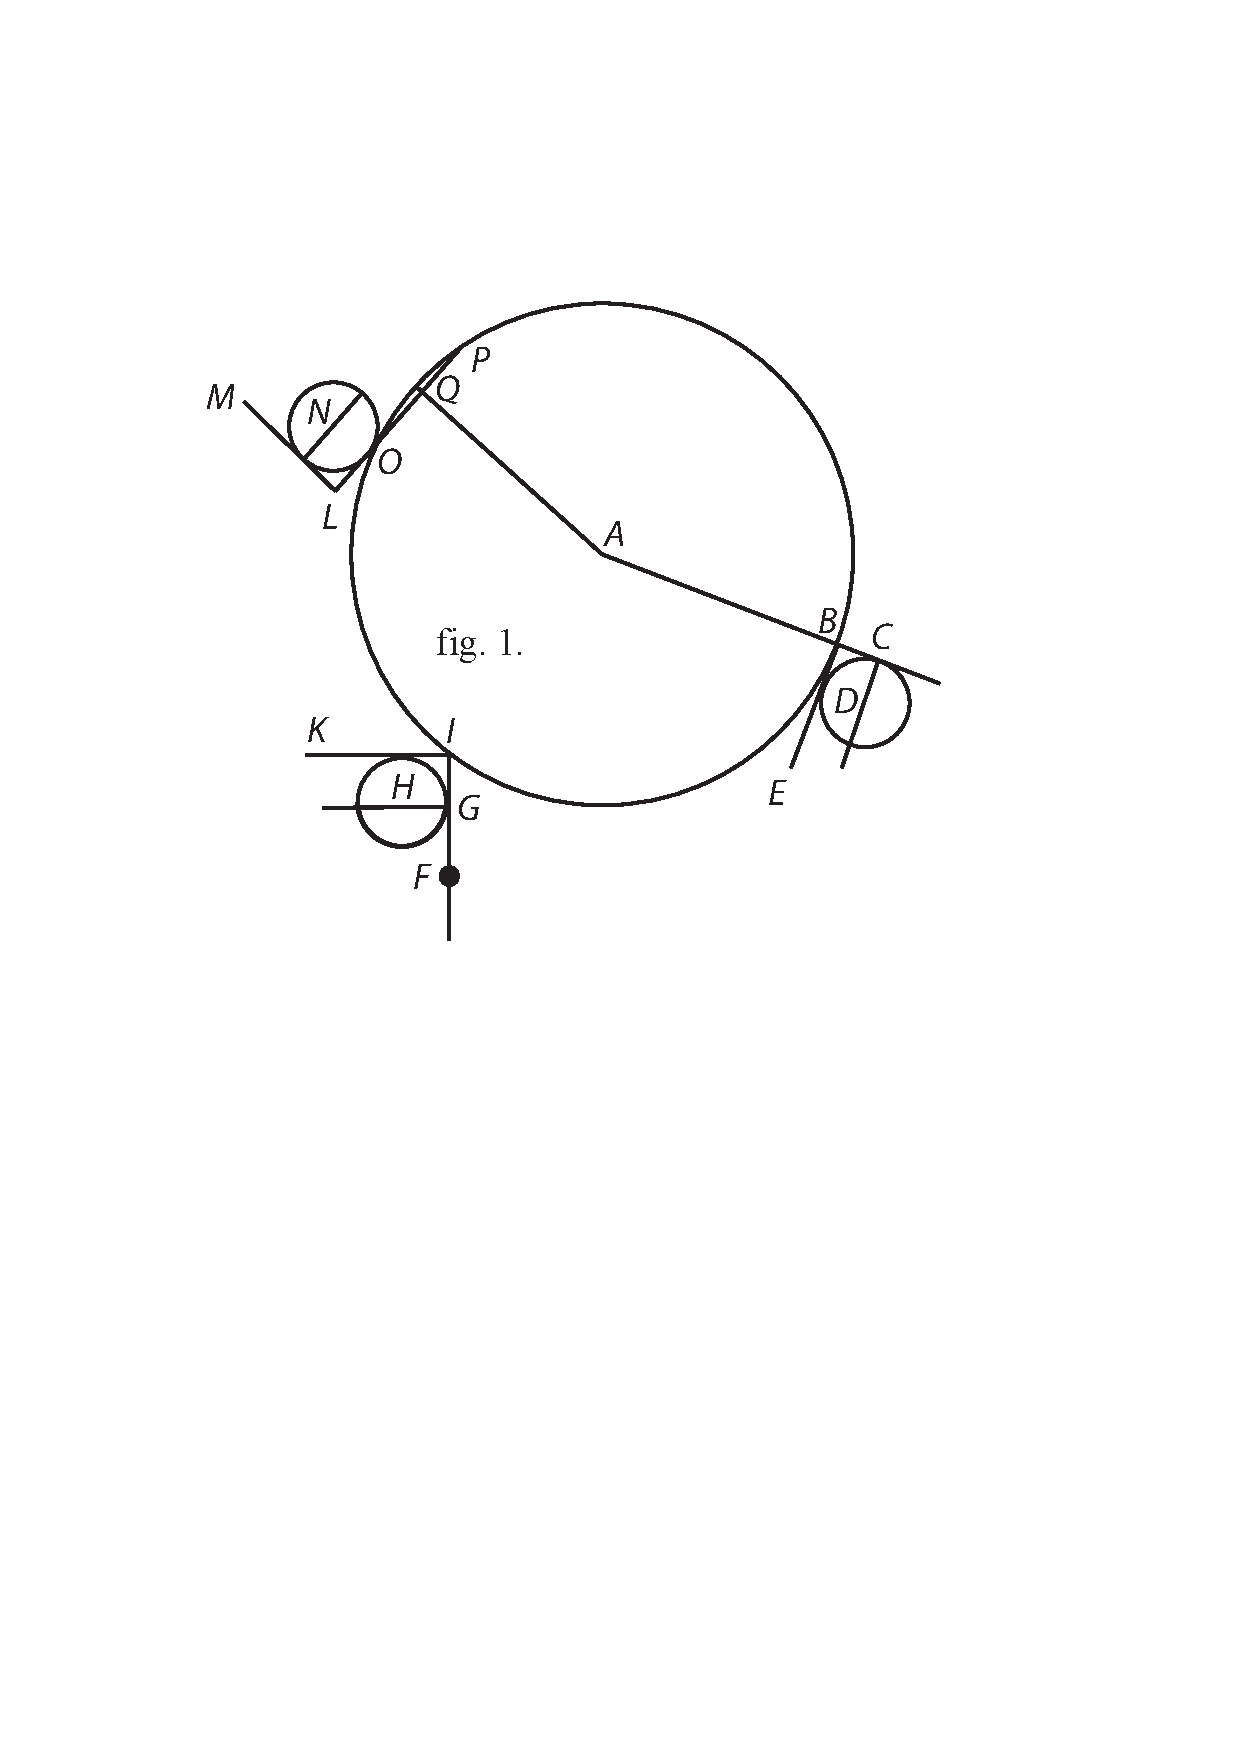
\includegraphics[width=0.5\textwidth]{images/LH0351402_103v-d1.pdf}\\
%\rule[0mm]{30mm}{0mm}[\textit{Fig. 1}]
%\end{wrapfigure} 
Nimirum si corpus unum \edtext{in}{\lemma{}\Bfootnote{in \textit{erg. L}}} aliud \edtext{impingat, non videndum}{\lemma{impingat,}\Bfootnote{\textit{(1)}\ nil refert \textit{(2)}\ non videndum \textit{L}}} quae sit linea directionis, sed quem linea directionis angulum faciat ad corporis superficiem. Ita fieri poterit ut ejusmodi eminentiae in corpus subito incurrentes id faciant accedere versus centrum. Haec examinanda. Item alia de \edtext{lineis}{\lemma{de}\Bfootnote{\textit{(1)}\ figuris \textit{(2)}\ lineis \textit{L}}} directionis physicis, ut si corpus aliquod in aere volitans vel in aqua natans vel in terra positum, ictum\protect\index{Sachverzeichnis}{ictus} accipiat quid secuturum. An vera quae et ego et ille dicunt de linea ad centrum gravitatis\protect\index{Sachverzeichnis}{centrum gravitatis} ducta. Videndum scilicet si linea directionis perpendicularis ad superficiei planum tangens producta non tangat in centrum gravitatis an nihilominus vim exerceat ad corpus totum loco pellendum. Subtilis inquisitio putem utique cum in centrum gravitatis\protect\index{Sachverzeichnis}{centrum gravitatis} impingit recta impellere, sin aliter compositum fore motum ex recto et circulari, verum non circa centrum gravitatis, sed circa maxime remota +). 
\pend 
%\vspace{2em}
\pstart
\centering 
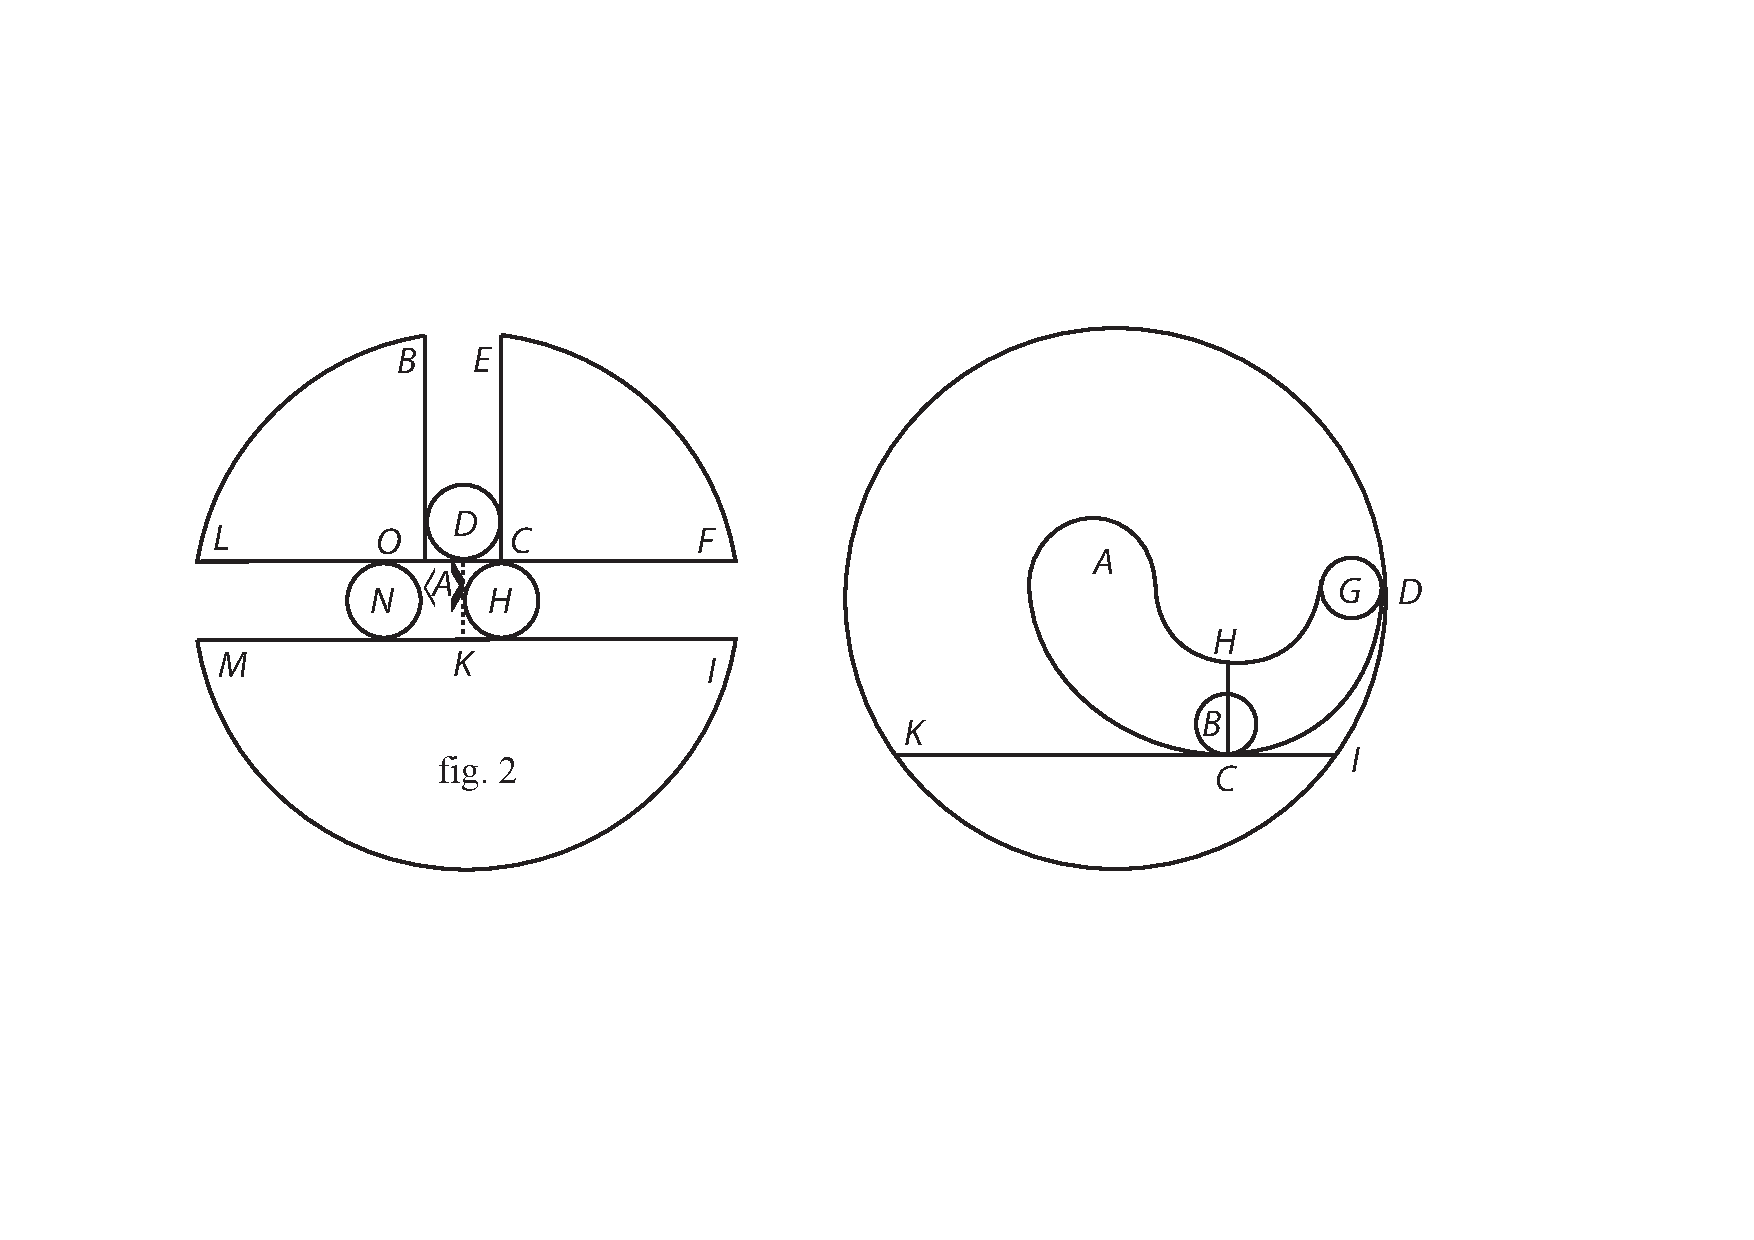
\includegraphics[width=1.0\textwidth]{images/lh0351402_103v23.pdf}
\pend
\vspace{0.5em}
\pstart
\hspace{20mm}[\textit{Fig. 2}]\edtext{}{\lemma{\hspace*{1,7mm}[\textit{Fig. 2}]}\killnumber\Cfootnote{Vgl. die Abbildung \cite{00326}a.a.O., S.~78.}} \hspace{54mm} [\textit{Fig. 3}]\edtext{}{\lemma{[\textit{Fig. 3}]}\killnumber\Cfootnote{Vgl. die Abbildung \cite{00326}a.a.O., S.~80.}}
\pend 
%\newpage
\vspace{2em}
\pstart
Alia \setline{1}figura\edtext{\textso{ fig. 2.}}{\lemma{\textso{fig. 2.}}\Bfootnote{\textit{erg. L}}}
in qua centrum \textit{A}[,] diameter \textit{AK}, sphaera\protect\index{Sachverzeichnis}{sphaera}
movetur super centro \textit{A} secundum puncta \textit{B E F L}[,]
globus mox ex \textit{D} in \textit{B}; ex \textit{H} in \textit{F}, ex \textit{N} in \textit{K} ibit,
quia primus casus ad praecedentis figurae casum primum,
secundus ad primae figurae casum secundum,
tertius ad casum ejusdem tertium
\edtext{pertineat.}{\lemma{pertineat.}\Cfootnote{\cite{00326}a.a.O., S.~78f.}}
%
\textit{Si vero\textso{ fig. 3. }in sphaera \textit{DEF} excavetur canalis \textit{ABCD},
cujus latus \textit{ACD} sit helix,
dicta sphaera super \textit{A} revoluta globus \textit{G} semper ad centrum accedet
donec in \textit{A}
\edtext{quiescat.}{\lemma{quiescat.}\Cfootnote{\cite{00326}a.a.O., S.~79.}}}
%
Pone enim nunc esse v.g. in \textit{C} ducta tangente globi, \textit{KCI}, lineam \textit{CH}
(+~quae ad tangentem perpendicularis est~+)
motum globi designantem semper ad partes \textit{A} tendere
\edtext{comperiemus.}{\lemma{comperiemus.}\Cfootnote{\cite{00326}a.a.O., S.~79f.}}
%
(+~Haec Nulandius.\protect\index{Namensregister}{\textso{Nylandt} (Nulandius), Franz Wilhelm Frhr. von, 17. Jh.}
Vellem experimentum\protect\index{Sachverzeichnis}{experimentum} se fecisse dixisset.~%
\edtext{[\phantom(\hspace{-1.2mm}+)]}{\lemma{\phantom(\hspace{-1.2mm}+)}\Bfootnote{\textit{erg. Hrsg.}}}
%
Ait se \edtext{de}{\lemma{de}\Bfootnote{\textit{erg. L}}}
regulis suis Hugenio\protect\index{Namensregister}{\textso{Huygens} (Hugenius, Ugenius, Hugens, Huguens), Christiaan 1629-1695}
scripsisse, qui suas jam dedisse publico
\edtext{significarit.}{\lemma{significarit.}\Cfootnote{Siehe \cite{01118}\textsc{C. Huygens}, \glqq Règles du mouvement dans la rencontre des corps\grqq, \textit{JS}, 18. März 1669, S.~22-24 (\cite{00113}\textit{HO} VI, Nr.~1716, S.~S.~383-386).}}
Interea et se ostendisse
\edtext{tractatum Joh. Alph. Borelli,\protect\index{Namensregister}{\textso{Borelli} (Borellus), Giovanni Alfonso 1608-1679}%
}{\lemma{tractatum [...] Borelli}\Cfootnote{Siehe \cite{01001}\textsc{G.A. Borelli}, \textit{De vi percussionis}, Bologna 1667.}}
%
\textit{qui} inquit,
\textit{quanquam in plerisque nobiscum consentiat,
nonnullos tamen paralogismos\protect\index{Sachverzeichnis}{paralogismus} effugere non
\edtext{potuit.}{\lemma{potuit.}\Cfootnote{\cite{00326}\textsc{F.W. Nylandt}, \textit{Elementa physica}, S.~83.}}}
\pend 
\pstart  
Regulae motus Nulandii\protect\index{Namensregister}{\textso{Nylandt} (Nulandius), Franz Wilhelm Frhr. von 17. Jh.}: \textit{(1) Si duo corpora aequalia, aequali celeritate mota, sibi mutuo occurrant, resilient nulla celeritatis parte omissa. 2. Si duo corpora aequalia, inaequali celeritate mota sibi mutuo occurrant, id quod tardius movetur, alteri de sua celeritate nihil largiri potest. 3. Sed nec id quod celerius movetur alteri totum suum motum communicare est potens. 
%\left
$\langle4.\rangle$ Si duo corpora aequalia inaequali celeritate mota sibi mutuo occurrant resilient, eritque motus quem celerius motum alteri tard$\langle$io$\rangle$ri communicat ad motum suum totum in ratione celeritatis ad celeritatem. 5. Si sint duo corpora }\edtext{\lbrack\textit{aequalia}\rbrack}{\lemma{}\Bfootnote{\textit{aequalia} \textit{erg. Hrsg. nach Vorlage}}} \textit{quorum alterum infinities celerius moveatur, postquam sibi mutuo occurrerunt, illud quod celerius movebatur quiescet omnem suum motum alteri communicando. 6. Si duo corpora sint inaequalia, $\langle$min$\rangle$us vero celerius moveatur in ratione qua alterum illo est majus post occursum reflectetur nulla celeritatis parte amissa. 7. Si duo corpora $\langle$sin$\rangle$t in quavis ratione data, minus autem infinities celerius moveatur, si nempe alterum quies\-cat, illud quantumvis ingens $\langle$impe$\rangle$llet. $\langle$8.~Si~ra$\rangle$tio fuerit aequalitatis corpus motum quiescet totum suum motum alteri communicando. 9) Si vero id quod movetur mi$\langle$nus$\rangle$ sit r$\langle$eflect$\rangle$etur parte suae celeritatis amissa quam alteri largietur. 10) Si vero majus in eandem partem movebitur, parte quoque suae celeritatis amissa, quam alterum in se recipiet.}\edtext{}{\lemma{\textit{recipiet}.}\Cfootnote{a.a.O., S. 84-86.\cite{00326}}}
\pend
\count\Bfootins=1500
\count\Cfootins=1500
\count\Afootins=1500